
%%%%%%%%%%%%
% Preamble %
%%%%%%%%%%%%
\documentclass{article}

\usepackage{lmodern}
\usepackage{microtype}
\usepackage[margin = 1in]{geometry}
\usepackage{titling}
\usepackage{caption}
\usepackage{subdepth}
\usepackage{fancyhdr}

\usepackage{amsmath}
\usepackage{amssymb}
\usepackage{mathtools}
\usepackage{dsfont}
\usepackage{bm}

\usepackage{enumitem}
\usepackage{listings}
\usepackage{graphicx}
\usepackage{booktabs}

\pagestyle{fancy}
\lhead{\thetitle}
\rhead{\theauthor}

\setlength{\droptitle}{-6em}
\setlength{\captionmargin}{8em}

\lstset{xleftmargin = 2em,
        xrightmargin = 2em,
        basicstyle = \footnotesize\ttfamily,
        numberstyle = \tiny,
        stepnumber = 2,
        showstringspaces = false}

%%%%%%%%%%%%%%%%%%%%%%%%
% ----- Commands ----- %
%%%%%%%%%%%%%%%%%%%%%%%%

% ----- Unbindngs -----

% Built-in probability operator:
\let\Pr\relax%

% Slashed O:
\let\O\relax%

% Built-in complex part operators:
\let\Re\relax%
\let\Im\relax%

% Built-in vector notation:
\let\vec\relax%

% ----- Probability Operators -----
\DeclareMathOperator{\Pr}{\mathds{P}}
\DeclareMathOperator{\E}{\mathds{E}}
\DeclareMathOperator{\Var}{Var}
\DeclareMathOperator{\Cov}{Cov}
\DeclareMathOperator{\Cor}{Cor}

\newcommand{\dP}{\df{\mathds{P}}}

\newcommand{\io}{\text{ i.o.}}
\newcommand{\ev}{\text{ ev.}}

\newcommand{\inD}{\mathop{\overset{\mathrm{d}}{\longrightarrow}}}
\newcommand{\inP}{\mathop{\overset{\Pr}{\longrightarrow}}}

\newcommand{\ind}{\protect\mathpalette{\protect\independenT}{\perp}}
\def\independenT#1#2{\mathrel{\rlap{$#1#2$}\mkern4mu{#1#2}}}

\newcommand{\dist}[1]{\operatorname{#1}}
\newcommand{\iid}{\overset{\mathrm{iid}}{\sim}}
\newcommand{\eqD}{\mathop{\overset{\mathrm{d}}{=}}}

% ----- Linear Algebra Operators -----
\DeclareMathOperator{\tr}{tr}
\DeclareMathOperator{\diag}{diag}
\newcommand{\vec}[1]{ \bm{\mathrm{#1}} }
\newcommand{\T}{ ^\mathsf{T} }

\newcommand{\1}{ \vec{1} }
\newcommand{\I}{ \vec{I} }

% ----- Calculus & Analysis Operators -----
\DeclareMathOperator*{\argmin}{argmin}
\DeclareMathOperator*{\argmax}{argmax}
\newcommand{\dv}[2][]{ \frac{\df{#1}}{\df{#2}} }
\newcommand{\pd}[2][]{\frac{\partial#1}{\partial#2}}
\newcommand{\df}[1]{ \mathop{\mathrm{d}#1} }

% ----- Constants & Sets -----
\DeclareMathOperator{\eul}{e}
\newcommand{\im}{\mathrm{i}}
\newcommand{\reals}{\mathds{R}}
\newcommand{\naturals}{\mathds{N}}
\newcommand{\integers}{\mathds{Z}}
%\DeclareMathOperator{\im}{i}

% ----- Functions -----
\DeclareMathOperator{\sinc}{sinc}
\DeclareMathOperator{\sign}{sign}
\DeclareMathOperator{\O}{\mathcal{O}}
\DeclareMathOperator{\Re}{\mathrm{Re}}
\DeclareMathOperator{\Im}{\mathrm{Im}}
\newcommand{\abs}[1]{\lvert#1\rvert}
\newcommand{\ceil}[1]{\lceil#1\rceil}
\newcommand{\floor}[1]{\lfloor#1\rfloor}

\newcommand{\on}[1]{\operatorname{ \mathds{1}}_\text{$#1$} }

% ----- Other Notations -----
\newcommand{\norm}[1]{\lVert#1\rVert}
\newcommand{\inner}[2]{\langle#1, #2\rangle}
\newcommand{\C}{^\mathsf{C}}

% Set up sentence-ending ellipses.
\def\ldotsplus{\mathinner{\ldotp\ldotp\ldotp\ldotp}}
\def\fourdots{\relax\ifmmode\ldotsplus\else$\m@th \ldotsplus\,$\fi}

\newcommand{\qed}{\hfill \ensuremath{\square}}

% Make the nice phi the default phi.
\let\temp\phi
\let\phi\varphi
\let\varphi\temp

%%%%%%%%%%%%
% Document %
%%%%%%%%%%%%
\title{The Frequency Domain Bootstrap}
\author{D. Izyumin, E. Shvarts, \& N. Ulle}
\date{Spring 2014}

\begin{document}
\maketitle

%%%%%%%%%%%
% Dmitriy %
%%%%%%%%%%%
\section*{Introduction}

\subsection*{Bootstrapping Time Series}
Since its introduction over three decades ago, the bootstrap has become a popular and widely applicable tool of statistical inference. At times, bootstrapping can provide valuable insight into the distributions of statistics, which would be unattainable by any analytical procedures. Over the years, numerous modifications and extensions of the original algorithm have made it possible to implement bootstrapping procedures in a variety of settings.

In the time series framework, observations are generally not independent and the dependence structure is a key object of interest. Moreover, there is usually an absence of repeated measurements, as only one realization of the process is observed. Since the bootstrap is based on the resampling of i.i.d objects, these two complications make the extension of the bootstrap to time series analysis a challenge.

The difficulties above may be overcome either by resampling whole blocks of observations (moving block bootstrap), or by first somehow transforming the data into i.i.d. objects and then resampling those. Examples of such i.i.d. transformations of the data are residuals and innovations in the time domain, or periodogram ordinates in the frequency domain. Dahlhaus and Janas outline a bootstrap procedure based on the resampling of Studentized tapered periodogram ordinates, and show that under reasonable assumptions the procedure has very favorable properties when dealing with an important class of ratio statistics \cite{bootstrap}.

\subsection*{Spectral Means and Ratio Statistics}

Consider a real-valued, stationary, zero-mean time series $\{X_t \}_{t\in\mathbb{Z}}$, of which realizations $t=1,\cdots,T$ are observed. The usual estimate of the spectral density function $f(\alpha)$ is the smoothed periodogram constructed from the observed data. For additional smoothing, the tapered periodogram, denoted by $I_T(\alpha)$, will be used instead. A brief motivation of tapering can be found in the \textit{Empirical Examples} section, and Dahlhaus and Janas provide a detailed description of the procedure in their publication.

For any $\phi = (\phi^{(1)},\cdots,\phi^{(d)})$, where each $\phi^{(i)}$ of bounded variation, the \textit{spectral mean} is defined as
	\[
	A(\phi, f) = \int_0^\pi \phi(\alpha)f(\alpha)d\alpha,
	\]
and the canonical estimate is given by
	\[
	A(\phi,I_T) = \int_0^\pi \phi(\alpha)I_T(\alpha)d\alpha
	\]

Now consider the normalized spectral density $g(\alpha) = \frac{f(\alpha)}{F(\pi)}$, where $F$ is the spectral distribution function. A natural estimate of this quantity is the normalized tapered periodogram, $J_T(\alpha)=\frac{I_T(\alpha)}{\hat{F}_T(\pi)}$, where $\hat{F}_T(\alpha)$ is the estimate of the spectral distribution function obtained using the tapered periodogram. The \textit{normalized spectral mean} is obtained when $g$ is plugged into $A(\phi,\cdot)$ in place of $f$,
	\[
	 A(\phi,g)=\frac{\int_0^\pi \phi(\alpha)f(\alpha)d\alpha}{\int_0^\pi f(\alpha)d\alpha} = \frac{A(\phi,f)}{A(1,f)},
	\]
and its estimate is obtained by similarly replacing $I_T$ by $J_T$,

	\[
	 A(\phi,J_T)=\frac{\int_0^\pi \phi(\alpha)I_T(\alpha)d\alpha}{\int_0^\pi I_T(\alpha)d\alpha} = \frac{A(\phi,I_T)}{A(1,I_T)}
	\]
Since the estimate can be expressed as a ratio of two spectral mean estimates, its is known as a \textit{ratio statistic}.


\subsection*{Examples}

The sample means and ratio statistics are both notable classes of statistics. Since it is only required that $\phi(\alpha)$ is bounded in variation, a great number of functions may be chosen for $\phi$, resulting in many different statistics and estimates. Below are several important estimates that can be expressed as either $A(\phi, I_T)$ or $A(\phi, J_T)$ with proper choice of $\phi$:\\

\begin{table}
\centering
\begin{tabular}{ccc}
\toprule
$\phi(\alpha)$ & $A(\phi,I_T)$ & $A(\phi,J_T)$ \\
\midrule
$\cos(\alpha u)$ & Autocovariance $\hat{\gamma}(u), u \in \mathbb{Z}$  &  Autocorrelation $\hat{\rho}_T(u), u \in \mathbb{Z}$ \\
$\on{[0,\lambda]}(\alpha)$ & Spectral Distribution Function $\hat{F}_T(\lambda)$ & Normalized SDF $\frac{\hat{F}_T(\lambda)}{\hat{F}_T(\pi)}$\\
\bottomrule
\end{tabular}
\caption{Useful spectral means and ratio statistics.}
\end{table}


\subsection*{Whittle Estimators}
Consider the problem of selecting a parameter $\theta$ from a parameter family $\Theta \in \mathbb{R}$ with the corresponding family of spectral densities $\mathcal{F}=\{f_\theta: \theta \in \Theta\}, \Theta \in \mathbb{R}$. The Whittle estimate of the parameter, $\hat{\theta}$, is obtained by minimizing Whittle's likelihood function,
	\[
	 \mathcal{L}_T(\theta) = \frac{1}{2\pi}\int_0^\pi \left[ \log f_\theta (\alpha) + \frac{I_T(\alpha)}{f_\theta(\alpha)} \right]d\alpha.
	\]
The likelihood $\mathcal{L}_T(\theta)$ can be interpreted as the distance between the (tapered) periodogram $I_T$ and the candidate spectral density $f_\theta$. In some settings Whittle estimates have very favorable properties and may be preferred over methods relying on the traditional likelihood \cite{fox}.

Notably, a Whittle estimator can be expressed as a spectral mean $A(\phi,I_T)$ with $\phi(\alpha) = \nabla \frac{1}{f_\theta}(\alpha)$. Using this fact, Dahlhaus and Janas extend their ideas to Whittle estimates, and show that their bootstrap algorithm has favorable properties when working with Whittle estimates as well.





%%%%%%%%%%
% Eugene %
%%%%%%%%%%
\section*{The Bootstrap Procedure}
%\subsection*{Resampling the Periodogram}
We are interested in approximating the distribution of ratio statistic estimates, and so need an estimator for the spectral mean $A(\phi,J_T)$ which we can compute via resampling. To this end, choose $n = \lfloor T/2\rfloor$, and consider $n$ equi-spaced samples of the periodogram, $I_j := I_T(\frac{j}{T/2}\pi)$ for $j=1,\ldots,n$. By resampling from (a carefully normalized version of) these values, we can obtain an appropriate discretization of the spectral mean. Letting $\{I_j^*\}$ be the $n$ resampled values, and $\phi_j := \phi(\frac{j}{T/2}\pi)$, consider
$$
B(\phi,I_T^*) := \frac{\pi}{n} \sum_{j=1}^n \phi_j I_j^*~~.
$$
Our interest is in the behavior of the approximation error $A(\phi,I_T) - A(\phi,f)$, and so we consider the corresponding quantity $B(\phi,I_T^*) - B(\phi,\hat f)$, where $\hat f$ is a suitable estimate for the spectral density (e.g., a consistent estimator formed from the periodogram values, perhaps via kernel smoothing). For the former, the (untapered) periodogram estimate obeys a central limit theorem (proved, e.g., in \cite{dahlhauslimitlaw}), such that $\sqrt T \bigl( A(\phi,I_T) - A(\phi,f)\bigr)$ is asymptotically normal with variance equal to $2\pi \int \phi^2 f^2 + (\kappa_4 / \sigma^4)\left(\int \phi f\right)^2~$. Here $\kappa_4$ and $\sigma^2$ refer to the fourth cumulant and variance of the innovations in the underlying presumed linear process. Additionally, in \cite{bootstrap}, it is stated that $\sqrt T \bigl( B(\phi,I_T^*) - B(\phi,\hat f)\bigr)$ is also asymptotically normal, with variance proportional to $2\pi \int \phi^2 f^2~$.

Hence, the latter statistic will only be useful for a bootstrap procedure if the second term in the former variance vanishes. Conveniently, this is fulfilled for example by Whittle estimates, and more generally by all ratio statistics. So, we will give an algorithm for resampling the periodogram which explains the `careful normalization' mentioned above. In particular, the quantities which we resample are Studentized, because we expect them to asymptotically vary as independent exponential variables. \cite{brillinger}[Theorem 5.2.6] \\

\textbf{Periodogram Bootstrap Algorithm} (of \cite{bootstrap})
\begin{enumerate}
\item Obtain the periodogram sample values $\{I_j\}$ for $j=1,\ldots,n$, possibly applying a taper to the data.
\item Obtain a consistent estimate $\hat f$ of the spectral density $f$, using the $\{I_j\}$. Kernel estimates are typical. 
\item Obtain Studentized periodogram samples $\hat\epsilon_j := I_j / \hat f_j$. 
\item Rescale the $\hat\epsilon_j$'s by their mean, so that $\tilde\epsilon_j := \hat\epsilon_j / \{(1/n) \sum_j \hat\epsilon_j\}$. This avoids unnecessary bias at the resampling stage. 
\item Sample the empirical distribution of $\{\tilde\epsilon_j\}$ to obtain a bootstrap sample $\{\epsilon^*_j\}$. 
\item Define bootstrap periodogram values via $I_j^* := \hat f_j \epsilon^*_j$.
\end{enumerate}

\subsection*{Assumptions}

In order to estimate the distribution of the approximation error $A(\phi,I_T) - A(\phi,f)$ by that of $B(\phi,I_T^*) - B(\phi,\hat f)$, the time series and desired spectral mean must be sufficiently nice; we describe some conditions and their relationship with the result. 
\begin{itemize}
\item First, $\{X_t:t\in\mathbb Z\}$ must be a real-valued linear process: $X_t = \sum_{u\in\mathbb Z} a_u \xi_{t-u}$. \\ The $\{\xi_t\}$ satisfy $\mathbb E \xi_1 = 0$, $\mathbb E \xi_1^2 = 1$, $\mathbb E \xi_1^8 <\infty$, $\mathbb E \xi_t^3 = 0$. The first two conditions are necessary for weak stationarity. Finite eighth moments are necessary for the bootstrap distribution to converge to the exponential distribution. \cite{bootstrap}[Corollary 1] Having vanishing third moments satisfies a technical constraint guaranteeing a good approximation of the relevant covariance matrix. \cite{bootstrap}[Remark 5] Without this, we cannot attain the claimed convergence rate. \\ The $\{a_t\}$ vanish exponentially; this is a requirement imposed by the use of Edgeworth expansions in the proof.
\item The estimate $\hat f$ of $f$ is uniformly strongly consistent, such that
$$
\sup_{\alpha\in[0,\pi]} |\hat f(\alpha) - f(\alpha)| \to 0 ~~\text{almost surely.}
$$
This is necessary for showing convergence in distribution. Further, the spectral density $f$ itself is everywhere-positive and bounded away from zero; in particular, there are no vanishing Fourier modes. 
\item $\phi$ is a $d$-dimensional vector of bounded-variation functions $\phi^{(r)}:[0,\pi]\to\mathbb R$, each with even periodic extension to all of $\mathbb R$. This broad definition allows for a rich choice of spectral means for estimating. The use of Edgeworth expansions further imposes that the Fourier coefficients $\{\hat \phi (\omega)\}$ vanish exponentially. While this would technically omit some important classes of statistics, this requirement is not sharp, and the method's validity beyond the theoretical guarantee is suggested by empirical evidence. 
\item The taper function has several technical limitations placed on it; the Tukey-Hanning tapers are given in \cite{bootstrap} as an example of an acceptable choice. The innovations $\{\xi_t\}$ and $\phi$ also must satisfy some technical conditions for the use of Edgeworth expansions. 
\end{itemize}

\subsection*{Convergence Rate}

Under the necessary assumptions, estimating the distribution of the standardized spectral density by resampling from the standardized periodogram is consistent, and the convergence rate is asymptotically better than that achieved by the normal approximation. 

To be precise, let $A(\phi,g)$ be the ratio statistic corresponding to the time series with spectral density $f$, $J_T$ be the corresponding standardized periodogram, $J_T^*$ be the bootstrapped periodogram, and $\hat g$ be an estimator of the normalized spectral density, defined according to $\hat g_j := \hat f_j / \{(\pi/n) \sum_k \hat f_k\}$. Denote $V_T$ as the covariance matrix of $\sqrt T A(\phi,J_T)$. Define $D_T$ according to $D_T^2 = V_T^{-1}$, and define $\hat D_T$ analogously via $\sqrt T B(\phi,J_T^*)$. Let $P^*$ denote the conditional probability given the data. Then, we have the result \cite{bootstrap}[Theorem 1]:\\

\textbf{Theorem:}
Suppose the necessary assumptions hold. Then for almost all samples $\{I_j\}$, 
$$
\sup_C \left| P\bigl( \sqrt T D_T(A(\phi,J_T) - A(\phi,g)) \in C \bigr) \right. - \left. P^*\bigl(\sqrt T \hat D_T(B(\phi,J_T^*)-B(\phi,\hat g)) \in C  \bigr)\right| = o(T^{-1/2})~~.
$$
The $\sup$ is taken over convex measurable subsets of $\mathbb R^d$.

%%%%%%%%
% Nick %
%%%%%%%%
\section*{Empirical Examples}
\subsection*{Practical Details}
A random process can only be observed over a finite span of time.
Consequently, the sample endpoints will typically interrupt any oscillations
at two distinct points in their cycle.
The discrete Fourier transform treats the sample as periodic,
and the resulting discontinuity at the endpoints generates noise,
or \textit{leakage}, in the periodogram.
Smoothing the tails of the sample towards zero,
a process known as \textit{tapering},
eliminates the discontinuity and can help to alleviate leakage.
Following the procedure of Dahlhaus and Janas,
a $10\%$ Tukey-Hanning taper was used for all examples presented here.
Small changes to the taper proportion had little, if any,
effect on the smoothed spectral density estimate $\hat{f}$.
In practice, other tapers can be used with the frequency domain bootstrap.
These were not investigated, to avoid distraction from our focus.

Although tapering reduces noise in the periodogram,
it isn't sufficient to make the periodogram a consistent estimator for the
spectral density.
This requires further smoothing.
In the examples, kernel smoothing is used, with the Epanechnikov kernel
    \[
    K(x) 
    = 
    \frac{3}{4}\pi \biggl[ 1 - \Bigl( \frac{x}{\pi} \Bigr)^2 \biggr].
    \]
Smoothing has a tendency to reduce or eliminate modes of the periodogram,
and care must be taken to preserve important details.
To this end, it's suggested to smooth the log-periodogram rather than smoothing
the periodogram directly.
Further bias correction is possible in light of the distribution of the
periodogram ordinates.
With kernel weights $w_j(x)$ defined in the standard way,
the smoothed, bias-corrected spectral density estimate is given by
    \[
    \hat{f}(x)
    =
    \exp\biggl[
        \sum_{j} w_j(x) \ln I_{j} 
        - \ln \Gamma\bigl(1 + w_j(x)\bigr)
    \biggr],
    \]
where $j = 0, \ldots, \floor{T / 2}$.
The bandwidth is also essential, 
and should be selected to offer a good compromise between noise reduction and
loss of detail.

\subsection*{Example 1}
Consider estimation of the lag-1 autocorrelation $\rho(1)$,
in the $\dist{AR}(1)$ model $X_t = 0.9 X_{t-1} + Z_t$,
using $T = 64$ observations.
The innovations $\{Z_t\}$ are independent and identically distributed
$\dist{U}(-\sqrt{3}, \sqrt{3})$ random variables,
making them a mean 0, variance 1 white noise.
In this setting, the conditions of Theorem~1 are satisfied.
A realization of this process is shown in Figure~\ref{ex1}.
    \begin{figure}[ht]
    \centering
    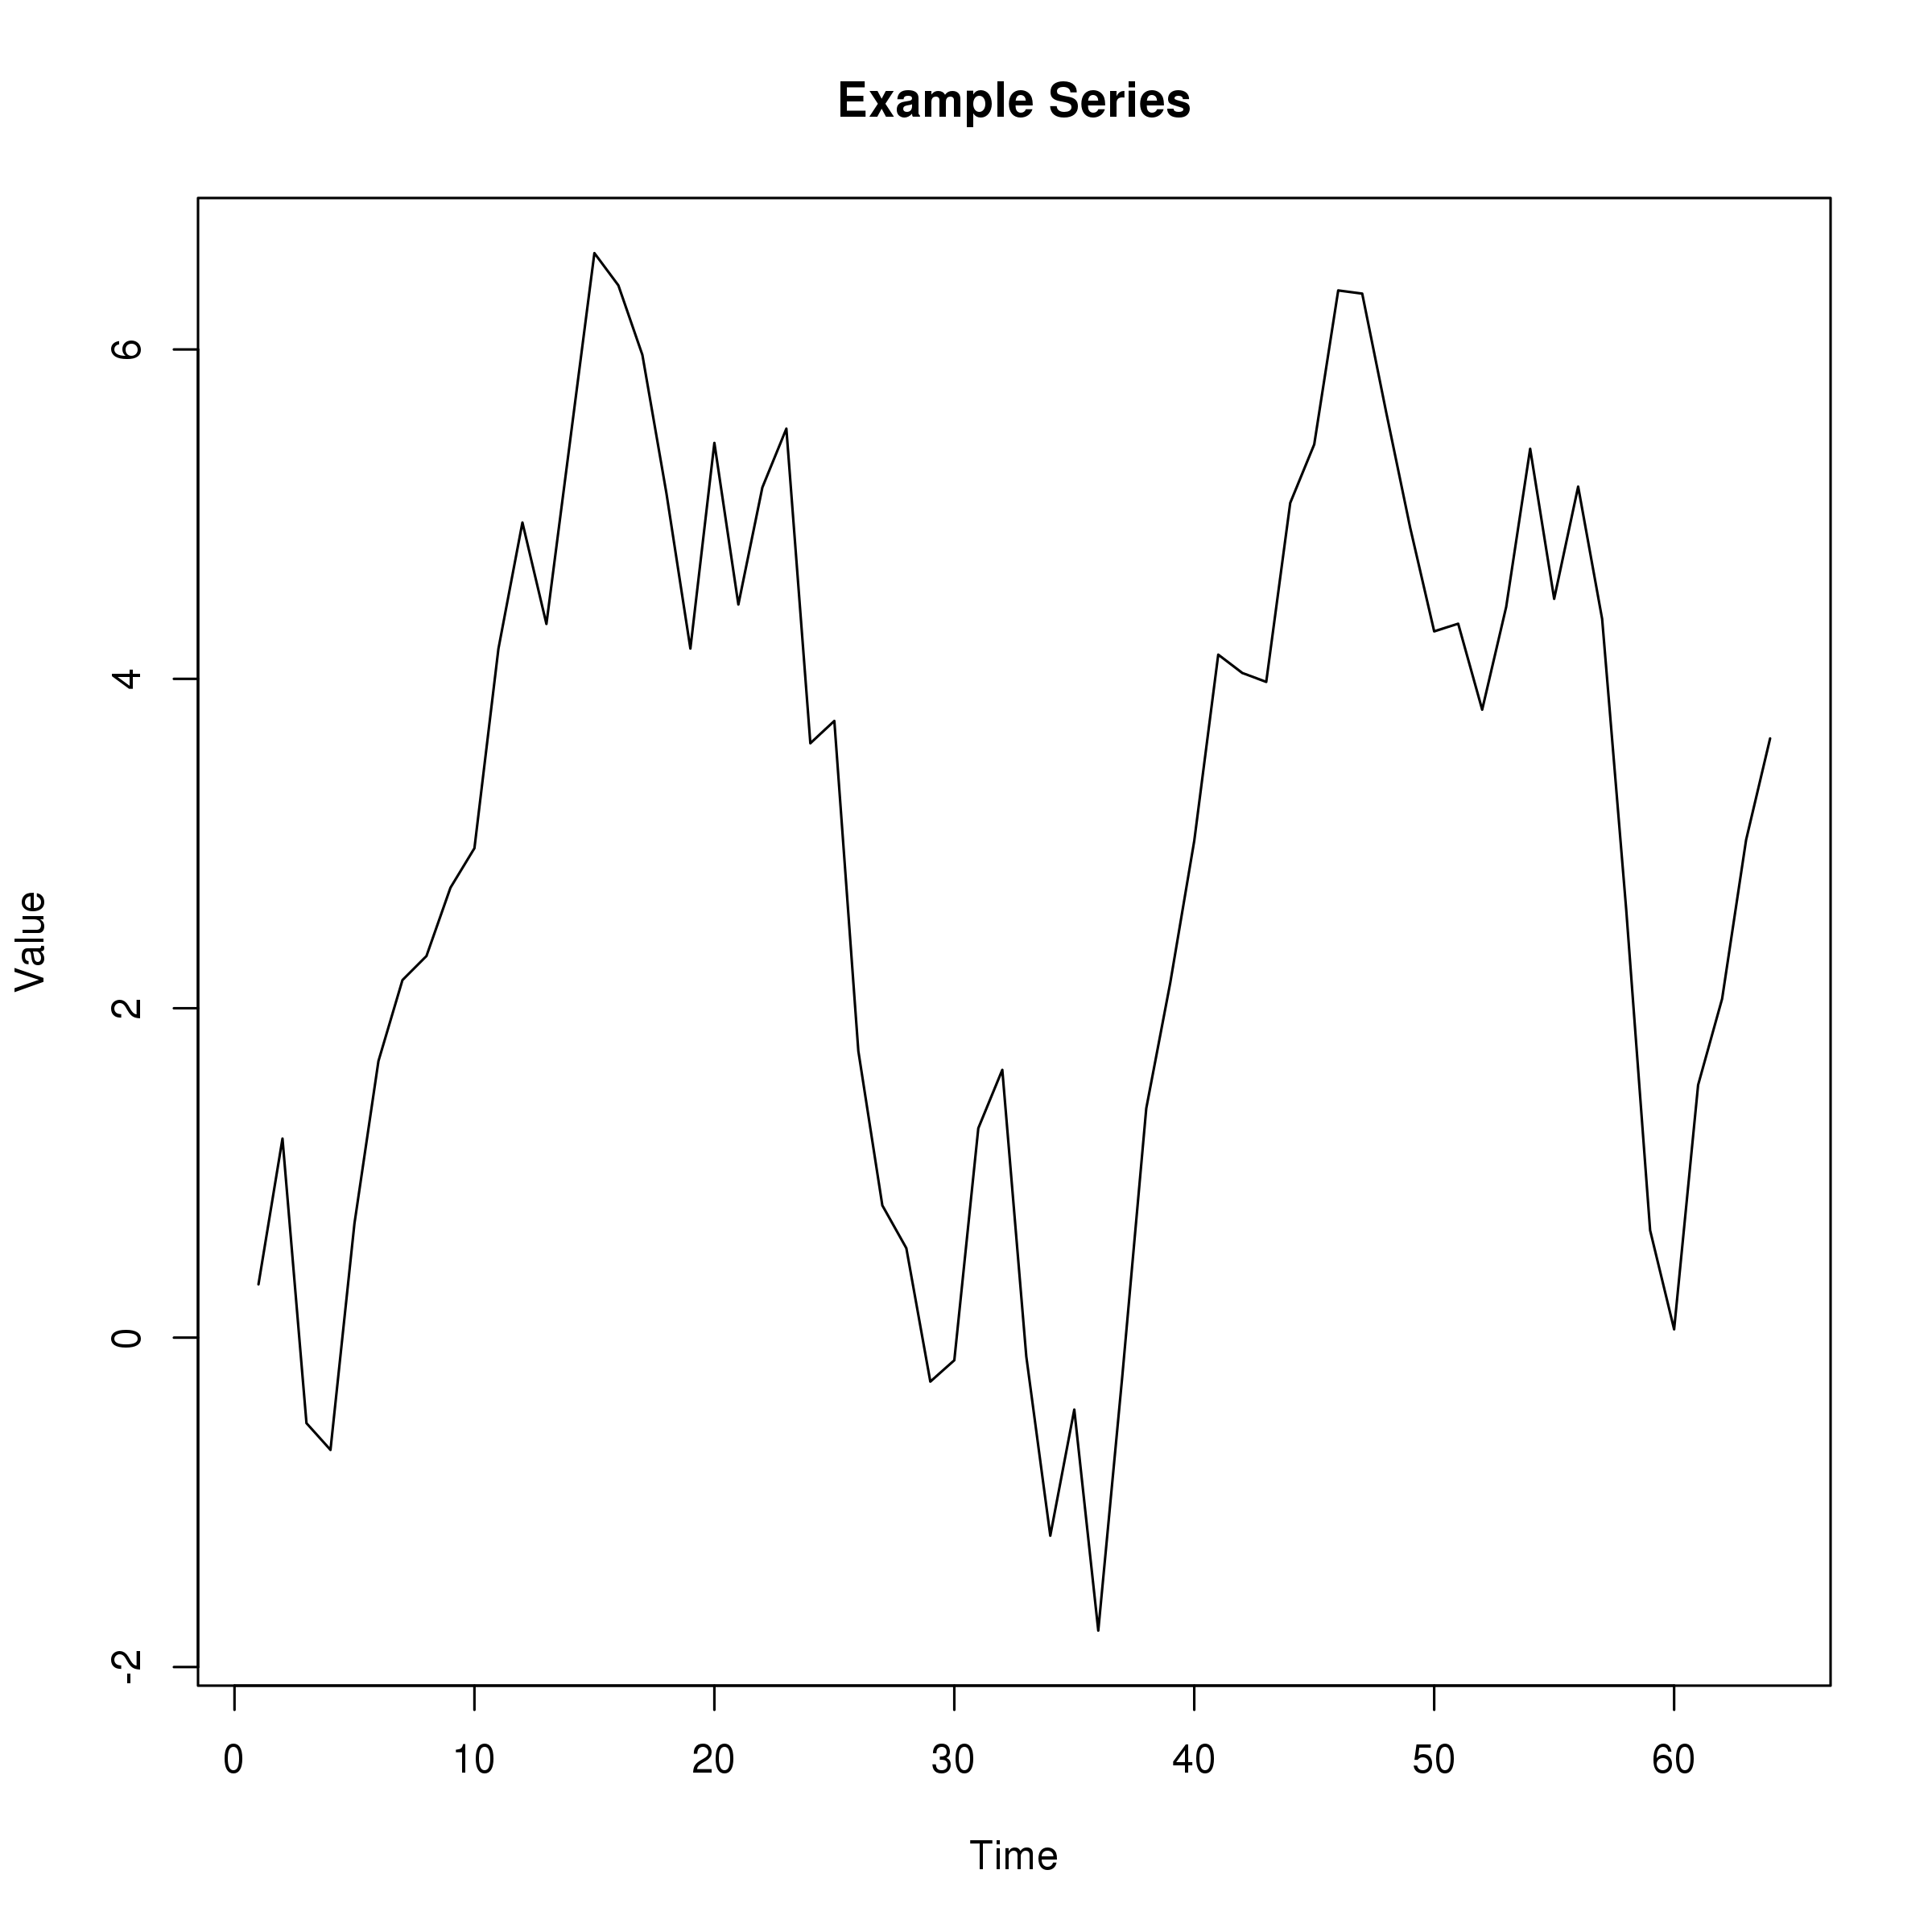
\includegraphics[width = 0.8\textwidth]{../res/ex1.png}
    \caption{
        A realization of the $\dist{AR}(1)$ process in Example 1.
        }
    \label{ex1}
    \end{figure}

A key feature of this model is that its spectral density exhibits a sharp
mode at zero.
This makes spectral density estimation challenging,
because of the trade-offs inherent in smoothing the periodogram.
Figure~\ref{ex1_spec} shows that with a bandwidth of $0.1$,
much of the mode's peak is lost.
On the other hand, reducing the bandwidth to $0.05$ produces a misleading,
bimodal estimate.
The former was selected for use here.
    \begin{figure}[ht]
    \centering
    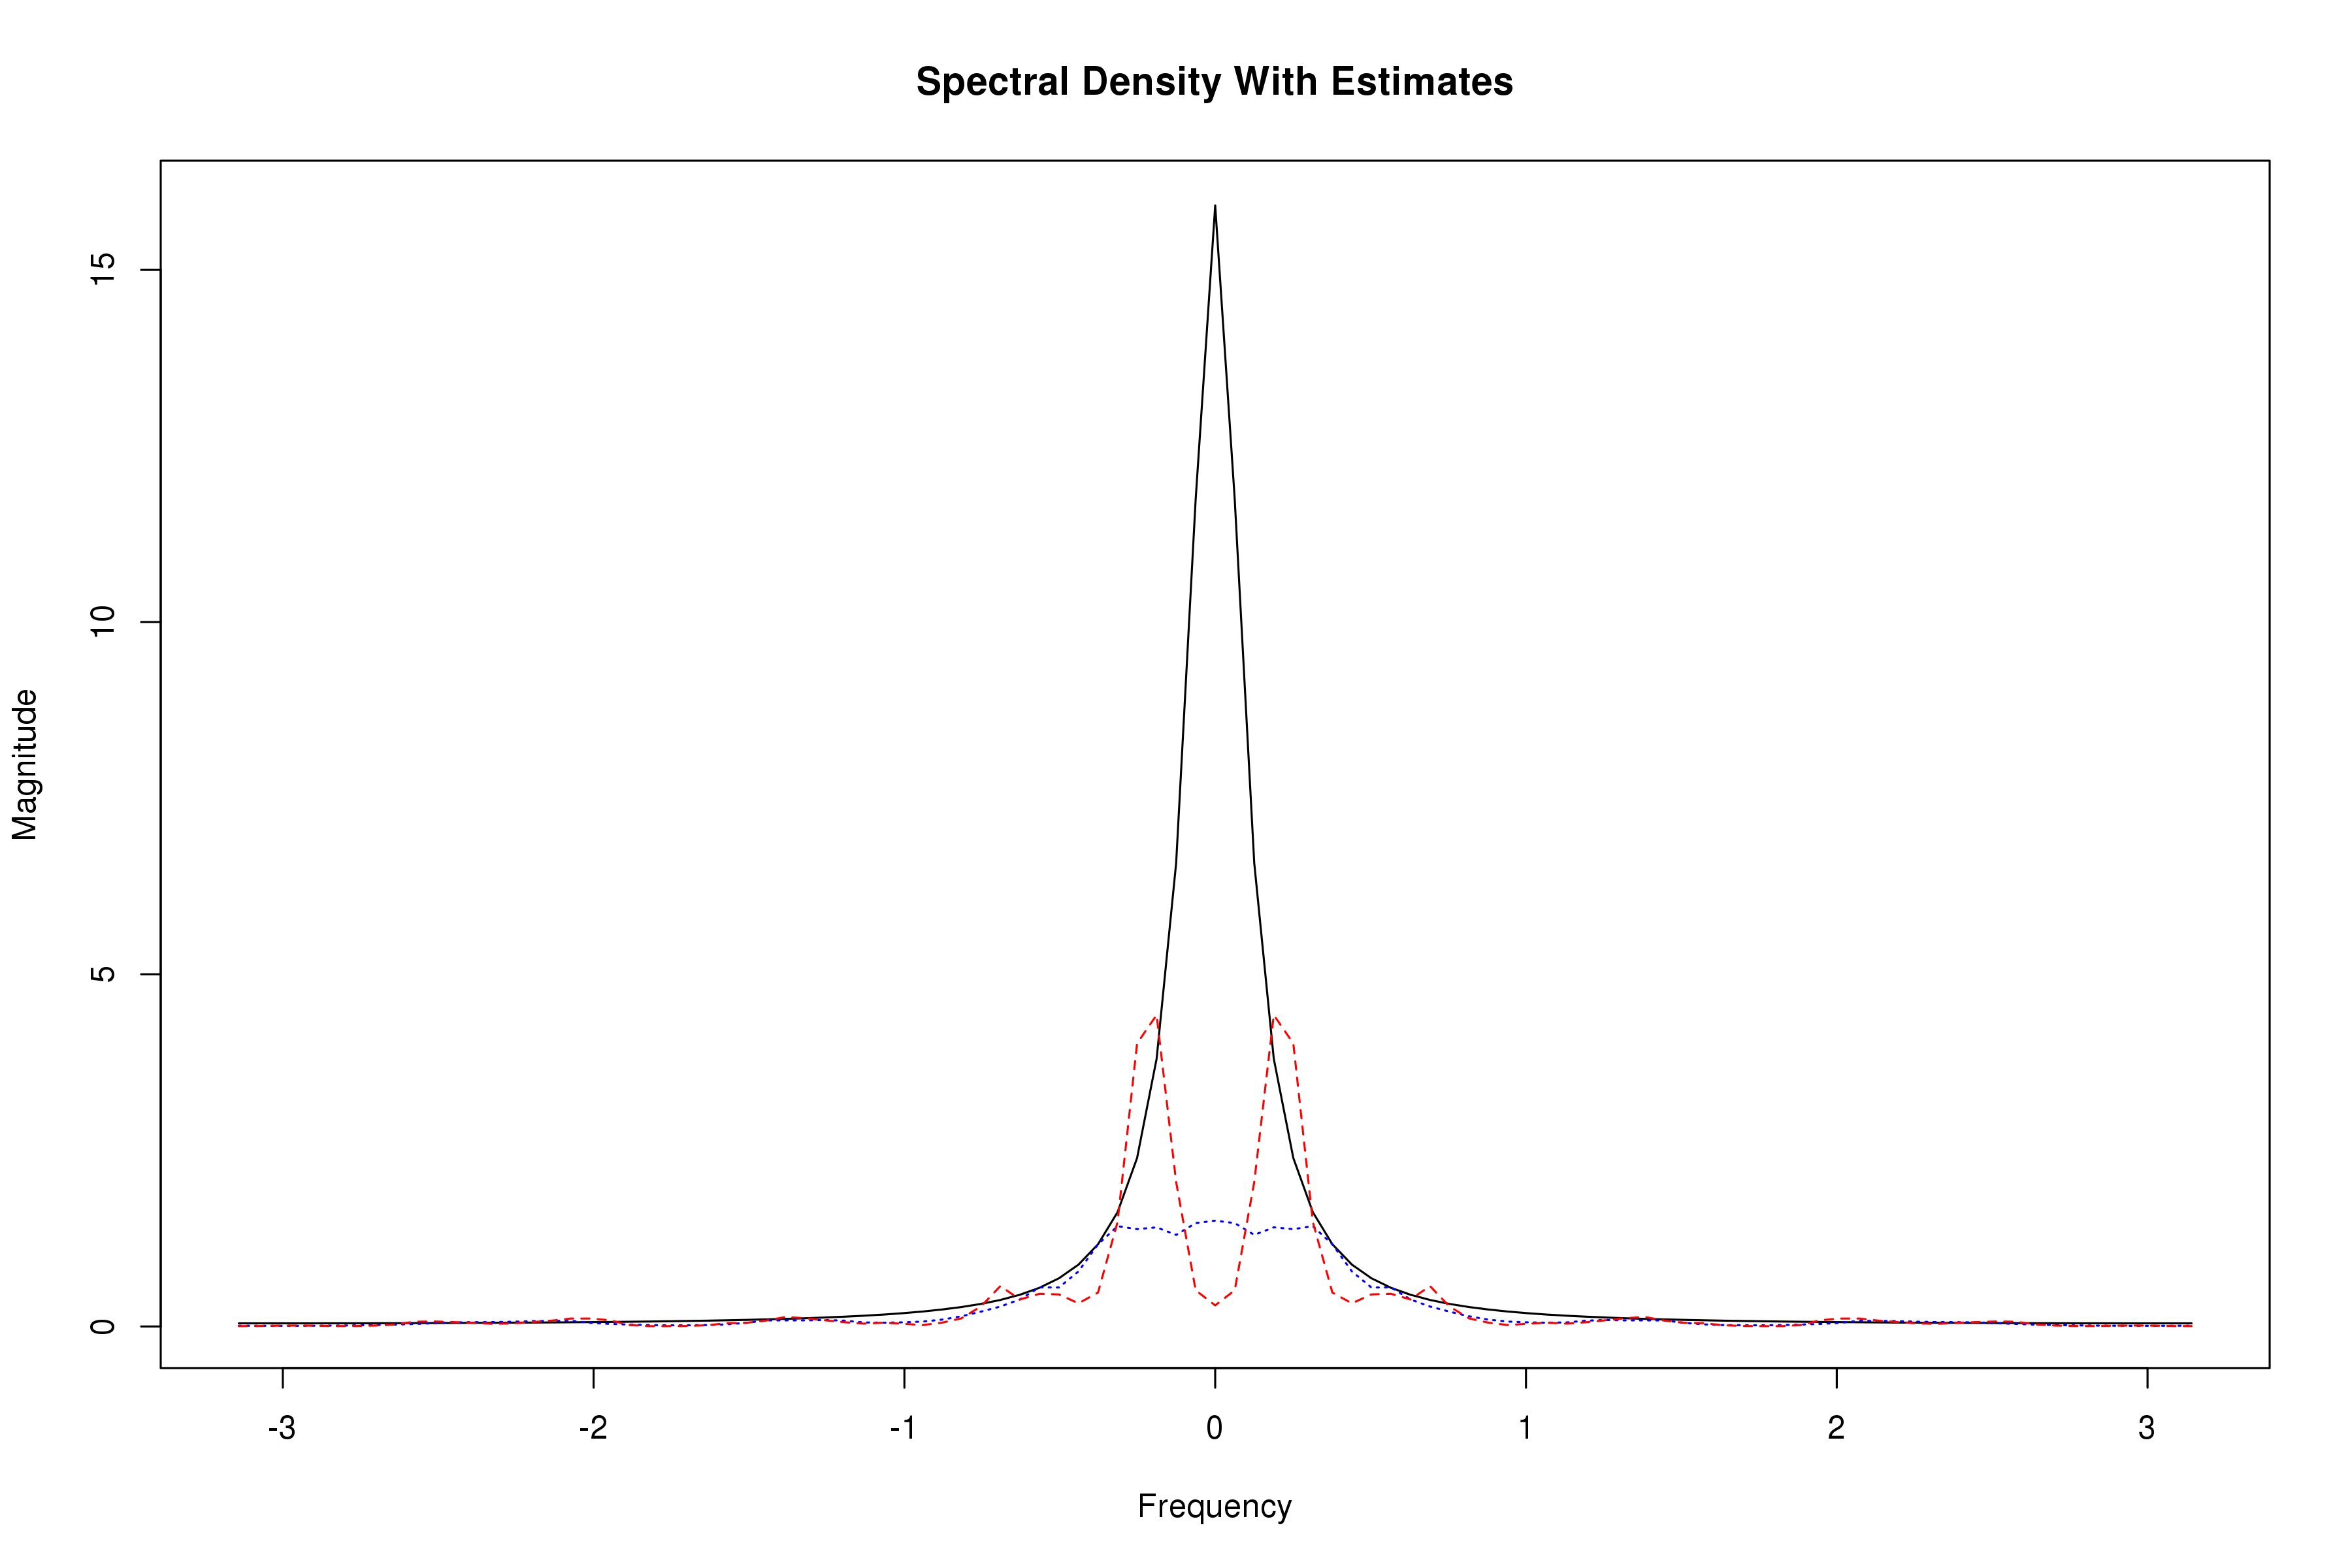
\includegraphics[width = 0.8\textwidth]{../res/ex1_spec.png}
    \caption{
        Example 1
        spectral density (solid, black) and spectral density estimates
        at bandwidth 0.1 (dotted, blue) and 0.05 (dashed, red).
        }
    \label{ex1_spec}
    \end{figure}

The estimate $\hat{\rho}(1)$ for the lag-1 autocorrelation $\rho(1)$
coincides with the Yule-Walker estimate of the AR parameter,
so we have the standard result that as $T \to \infty$,
    \[
        \sqrt{T} \biggl( \frac{\hat{\rho}(1) - 0.9}{c} \biggr)
        \inD
        \dist{N}(0, 1 - 0.9^2),
    \]
where $c$ is a correction for the taper.
This asymptotic error distribution is what would typically be used to construct
confidence bounds on the estimate.
The frequency domain bootstrap provides a bootstrapped error distribution as
a competitor. 
In this case, $2000$ estimates were bootstrapped.
Figure~\ref{ex1_cdf} shows a plot of the cumulative distribution functions for
both, as well as the true distribution (as approximated by repeated 
simulation).
The figure confirms the result of Theorem~1:
the bootstrapped distribution significantly outperforms the asymptotic
distribution.
This result is especially impressive because the spectral density estimate
was not very good---smoothing masked the peak at zero.
Repeated simulations show similarly positive results.
    \begin{figure}[ht]
    \centering
    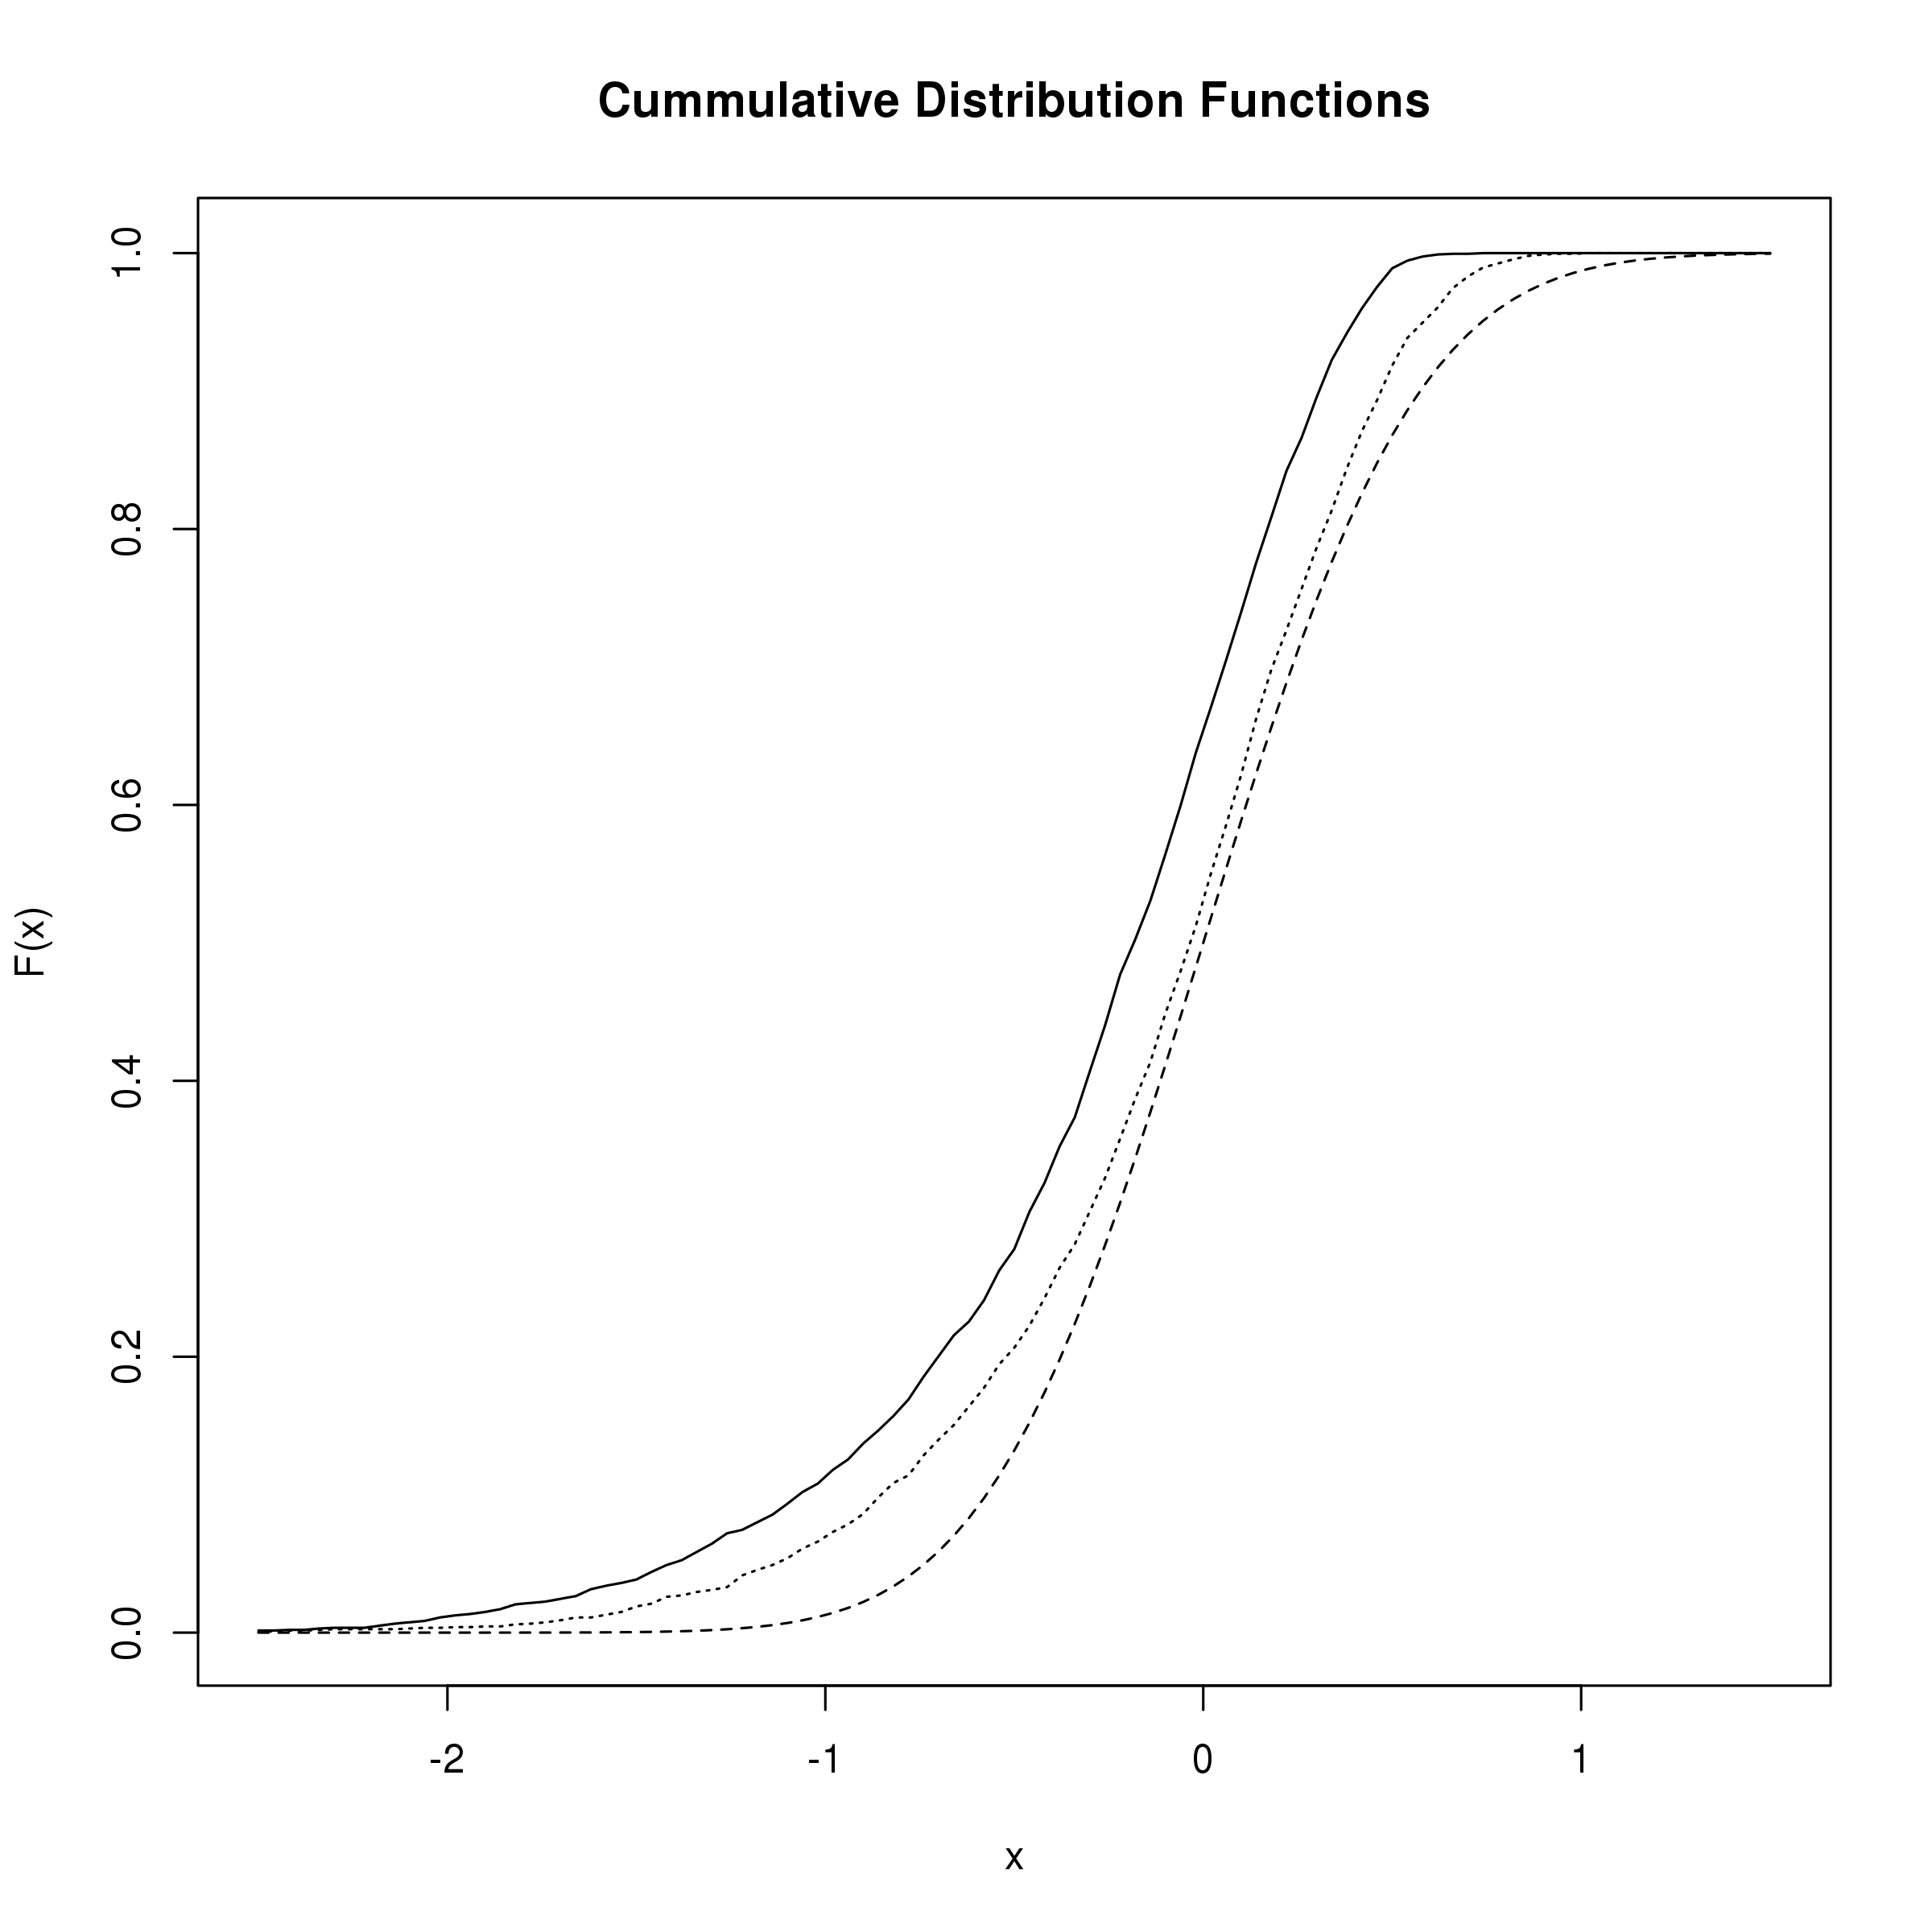
\includegraphics[width = 0.8\textwidth]{../res/ex1_cdf.png}
    \caption{
        Example 1
        CDFs for the true (solid, black), bootstrapped (dotted, blue),
        and asymptotic (dashed, red) error distributions.
        }
    \label{ex1_cdf}
    \end{figure}

\subsection*{Application}
    \begin{figure}[ht]
    \centering
    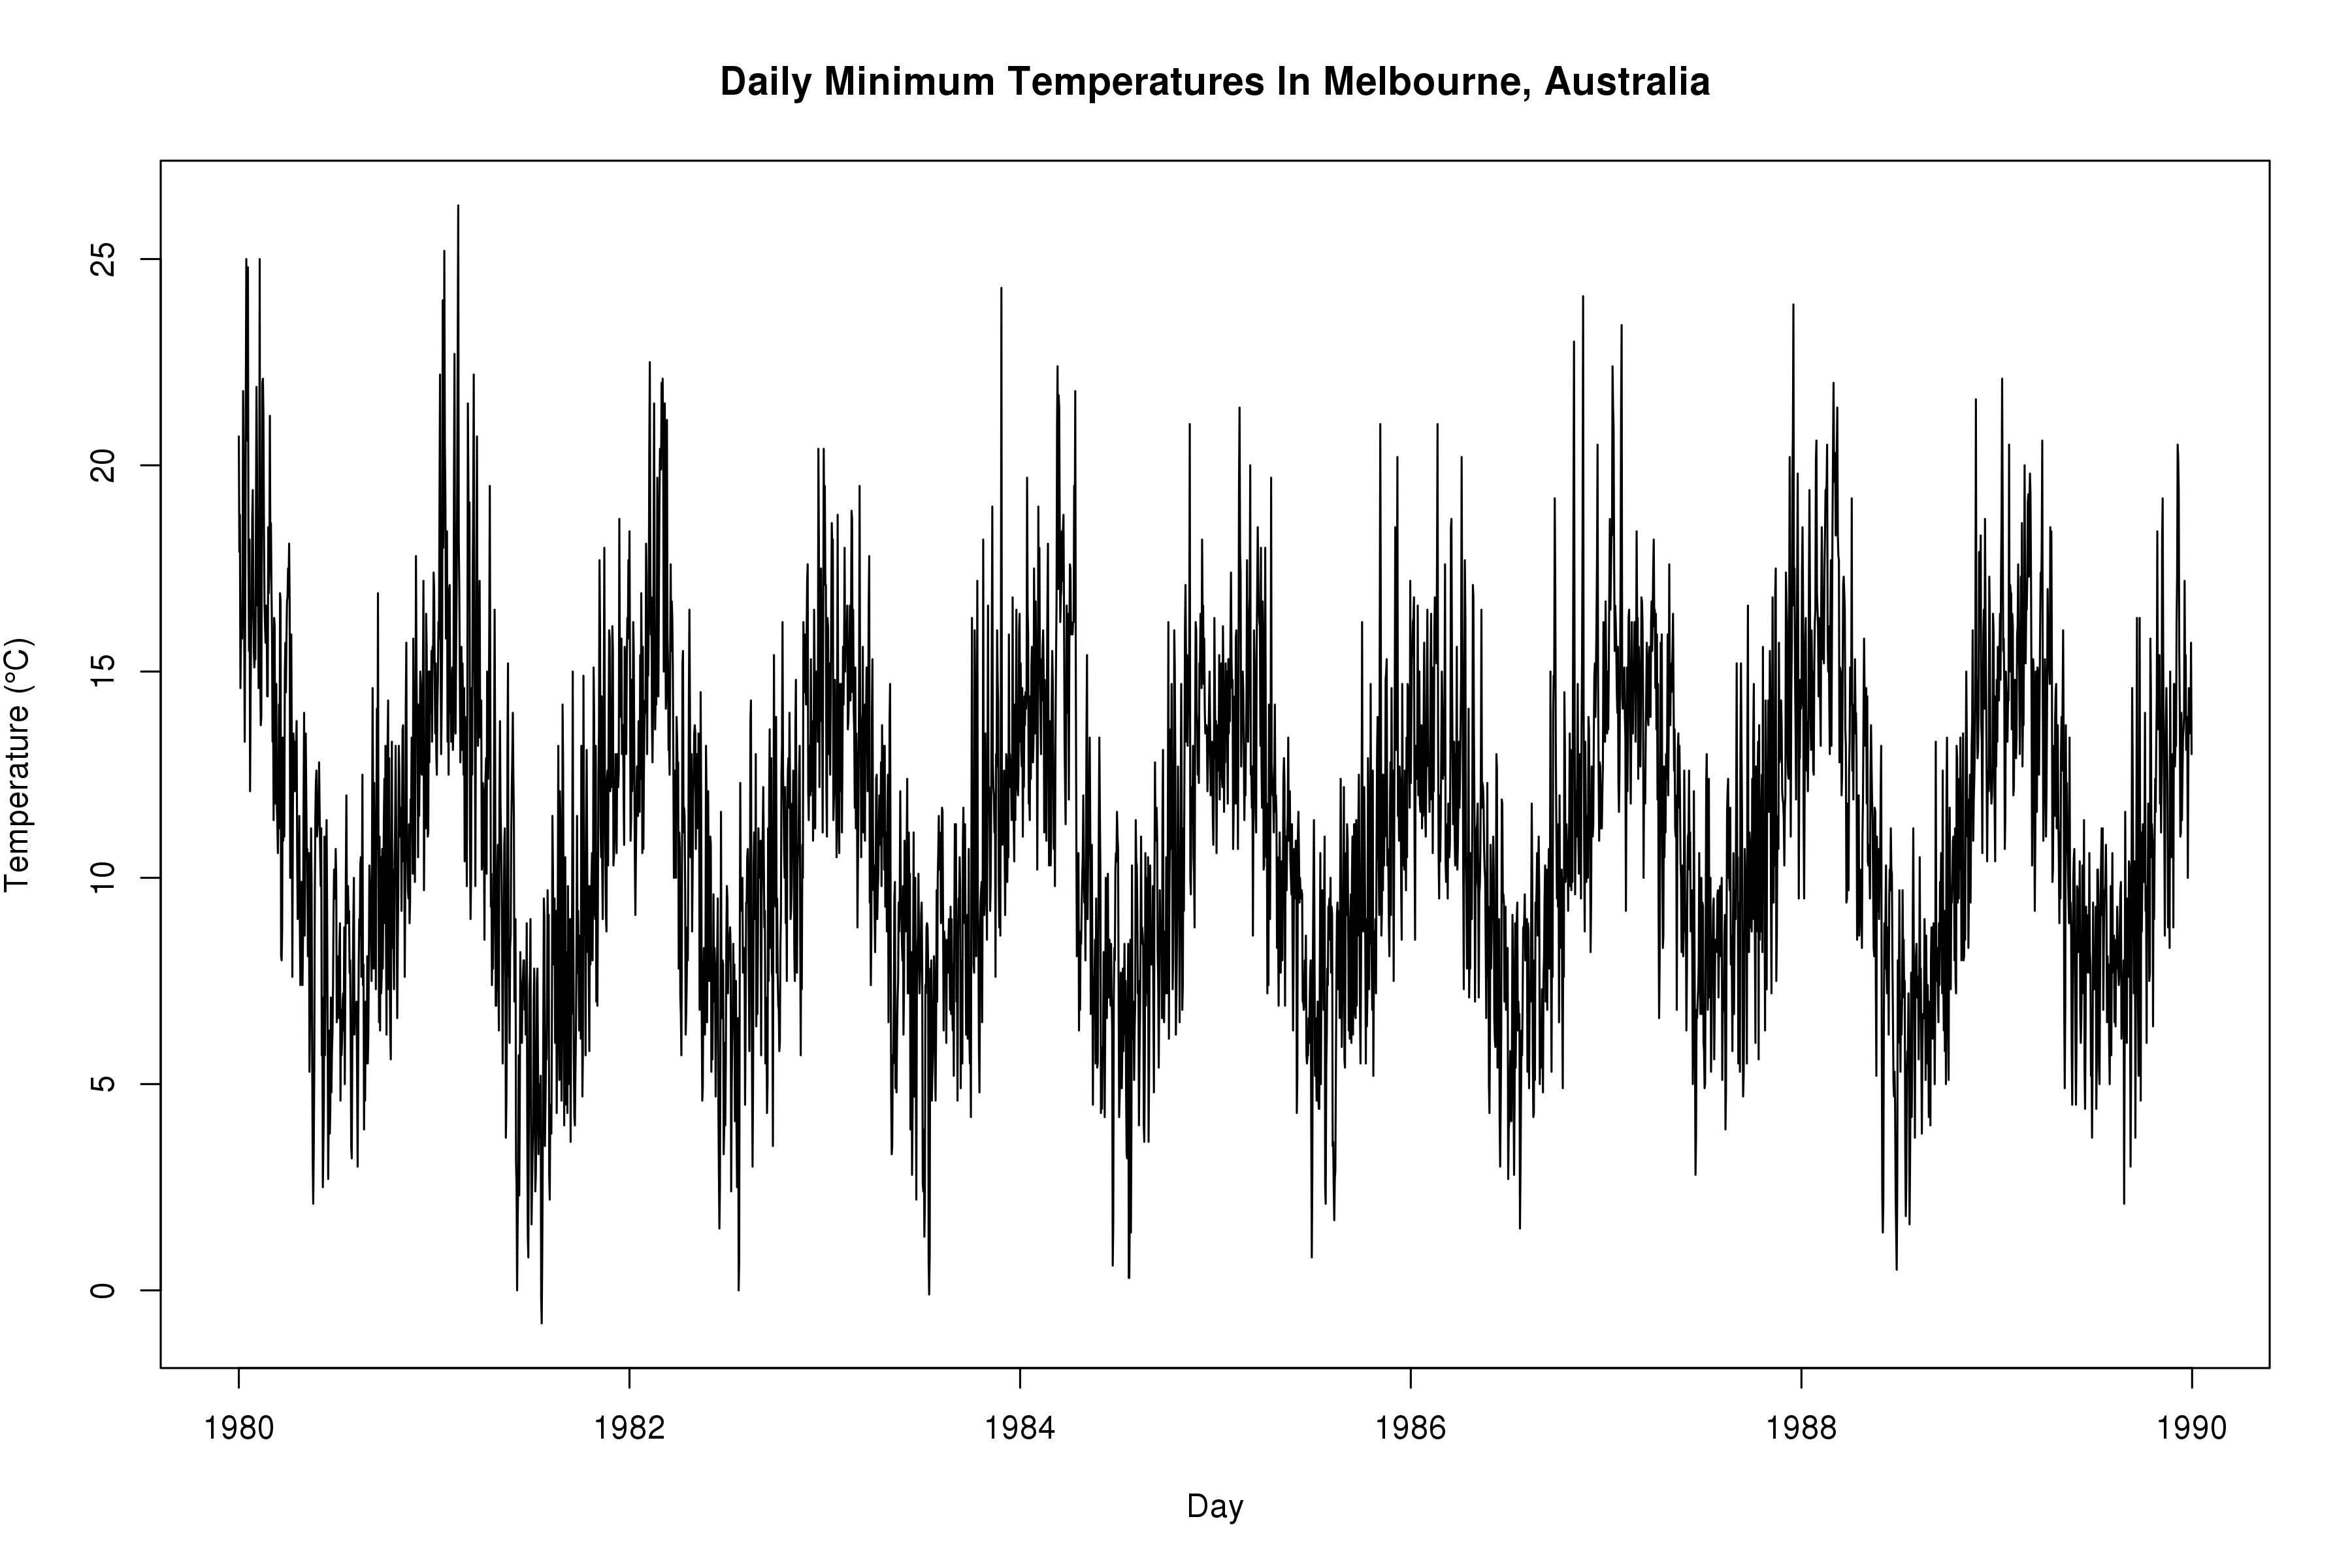
\includegraphics[width = 0.8\textwidth]{../res/exA.png}
    \caption{
        The Melbourne temperatures time series used in the application.
        }
    \label{ex1_cdf}
    \end{figure}


%%%%%%%%%%%%%%
% References %
%%%%%%%%%%%%%%
\bibliographystyle{plain} %we can also use, e.g., abbrv
\bibliography{237bib}

\end{document}
